%%%%%%%%%%%%%%%%%%%%%%%%%%%%%%%%%%%%%%%%%
% Beamer Presentation
% LaTeX Template
% Version 1.0 (10/11/12)
%
% This template has been downloaded from:
% http://www.LaTeXTemplates.com
%
% License:
% CC BY-NC-SA 3.0 (http://creativecommons.org/licenses/by-nc-sa/3.0/)
%
%%%%%%%%%%%%%%%%%%%%%%%%%%%%%%%%%%%%%%%%%

%----------------------------------------------------------------------------------------
%	PACKAGES AND THEMES
%----------------------------------------------------------------------------------------

\documentclass{beamer}

\mode<presentation> {

% The Beamer class comes with a number of default slide themes
% which change the colors and layouts of slides. Below this is a list
% of all the themes, uncomment each in turn to see what they look like.

%\usetheme{default}
%\usetheme{AnnArbor}
%\usetheme{Antibes}
%\usetheme{Bergen}
%\usetheme{Berkeley}
%\usetheme{Berlin}
%\usetheme{Boadilla}
%\usetheme{CambridgeUS}
\usetheme{Copenhagen}
%\usetheme{Darmstadt}
%\usetheme{Dresden}
%\usetheme{Frankfurt}
%\usetheme{Goettingen}
%\usetheme{Hannover}
%\usetheme{Ilmenau}
%\usetheme{JuanLesPins}
%\usetheme{Luebeck}
%\usetheme{Madrid}
%\usetheme{Malmoe}
%\usetheme{Marburg}
%\usetheme{Montpellier}
%\usetheme{PaloAlto}
%\usetheme{Pittsburgh}
%\usetheme{Rochester}
%\usetheme{Singapore}
%\usetheme{Szeged}
%\usetheme{Warsaw}

% As well as themes, the Beamer class has a number of color themes
% for any slide theme. Uncomment each of these in turn to see how it
% changes the colors of your current slide theme.

%\usecolortheme{albatross}
%\usecolortheme{beaver}
%\usecolortheme{beetle}
%\usecolortheme{crane}
\usecolortheme{dolphin}
%\usecolortheme{dove}
%\usecolortheme{fly}
%\usecolortheme{lily}
%\usecolortheme{orchid}
%\usecolortheme{rose}
%\usecolortheme{seagull}
%\usecolortheme{seahorse}
%\usecolortheme{whale}
%\usecolortheme{wolverine}

%\setbeamertemplate{footline} % To remove the footer line in all slides uncomment this line
%\setbeamertemplate{footline}[page number] % To replace the footer line in all slides with a simple slide count uncomment this line

\setbeamertemplate{navigation symbols}{} % To remove the navigation symbols from the bottom of all slides uncomment this line
}

\usepackage{graphicx} % Allows including images
\usepackage{booktabs} % Allows the use of \toprule, \midrule and \bottomrule in tables
\usepackage{hyperref}

\usepackage[utf8]{inputenc}
\usepackage[spanish]{babel}
\usepackage{listings}



%----------------------------------------------------------------------------------------
%	TITLE PAGE
%----------------------------------------------------------------------------------------

\title[Busqueda Binaria Recursiva]{Algoritmo de Busqueda Binaria Recursiva} % The short title appears at the bottom of every slide, the full title is only on the title page

\author{Grupo: Alias} % Your name
\institute[UTEM] % Your institution as it will appear on the bottom of every slide, may be shorthand to save space
{
Universidad Tecnológica Metropolitana \\ % Your institution for the title page
\medskip
\url{https://github.com/Lanceconan/AnalisisDeAlgoritmos} % Your site
}
\date{\today} % Date, can be changed to a custom date

\begin{document}

\setbeamercovered{transparent}

\begin{frame}
	\titlepage % Print the title page as the first slide
\end{frame}

\begin{frame}
	\frametitle{Introducción} % Table of contents slide, comment this block out to remove it
	\tableofcontents % Throughout your presentation, if you choose to use \section{} and \subsection{} commands, these will automatically be printed on this slide as an overview of your presentation
\end{frame}

%----------------------------------------------------------------------------------------
%	PRESENTATION SLIDES
%----------------------------------------------------------------------------------------

%------------------------------------------------
\section{Introduccion} % Sections can be created in order to organize your presentation into discrete blocks, all sections and subsections are automatically printed in the table of contents as an overview of the talk
%------------------------------------------------

	\subsection{Definición} % A subsection can be created just before a set of slides with a common theme to further break down your presentation into chunks

		\begin{frame}
			\frametitle{Definicion}
				\begin{center}
				La búsqueda binaria en un vector ordenado de datos se realiza comprobando el elemento que está en el centro del vector y mirando si el elemento buscado es mayor o menor. 
				\end{center}
		
		\end{frame}

		\begin{frame}
			\frametitle{Proposito búsqueda binaria}
				
			\begin{center}
			Se utiliza cuando el vector en el que queremos determinar la existencia de un elemento está previamente ordenado.

			Este algoritmo reduce el tiempo de búsqueda considerablemente, ya que disminuye exponencialmente el número de iteraciones necesarias.
			\end{center}
		\end{frame}


	\subsection{Funcion Binaria Recursiva en C/C++}

%------------------------------------------------

		\begin{frame}
			\frametitle{Funcion Binaria Recursiva en C/C++}
			\begin{figure}
  				\centering
    			           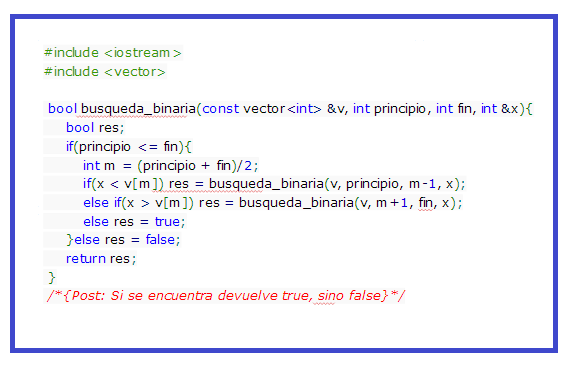
\includegraphics[scale=0.6]{CodigoC.png}
  				\caption{Codigo}
  				\label{fig:lls}
			\end{figure}
			
		\end{frame}

		
%------------------------------------------------
\section{Complejidad}
%------------------------------------------------

	\subsection{Calculo de Complejidad}

		\begin{frame}
			\frametitle{Calculo de complejidad}
			
		\end{frame}

%------------------------------------------------

	\subsection{Mejor Caso}

		\begin{frame}
			\frametitle{Mejor Caso}
			En base al árbol podemos postular que su altura esta expresada en la siguiente formula:
				\begin{equation}
					n < = 2^{(h + 1)} - 1
				\end{equation}
				Obteniendo que:
				\begin{equation}
					h >= \log_2{(n)}
				\end{equation}
				
			Esta es la característica principal de un árbol, la que permite que las operaciones sean tan rápidas, el único inconveniente es asegurar este mínimo valor para la altura ...
		\end{frame}
	\subsection{Peor Caso}
		\begin{frame}
			\frametitle{Peor Caso}
			Si sumamos las operaciones de inserción y recorrido tendriamos lo siguiente para el mejor caso:
			\begin{equation}
				O(n) = n  \log_2{(n)} + n
			\end{equation}
			O esto para el peor caso:
			\begin{equation}
				O(n) = n^2 + n
			\end{equation}
		\end{frame}

% Programa
\section{Sobre el programa}

	\subsection{Sobre el Código}
	\begin{frame}
		\frametitle{Sobre el Código}
			\begin{itemize}[<+->]
				\item IDE utilizado: Aptana Studio 3
				\item Programación en Ruby, version 1.9.3
				\item Una única clase con sus inherentes métodos
				\begin{itemize}[<+->]
					\item Métodos que permiten facil manipulación y entendimiento del código
					\item Variables Nemotécnicas
					\item Búsqueda binaria recursiva
				\end{itemize}
				\item Estructura utilizada: Un arreglo de largo N-1
				\item Metodo de Ordenamiento Burbuja (alternativo)
			\end{itemize}
	\end{frame}

	\subsection{Caracteristicas}
	\begin{frame}
		\frametitle{Caracteristicas}
			\begin{itemize}[<+->]
				\item Permite distintos poblamientos de los datos
				\begin{itemize}[<+->]
					\item Ordenado automatico (de entrada)
					\item Aleatorio
					\item Manual
				\end{itemize}
				\item Facil Manipulacion del Codigo
				\item Utiliza el ordenamiento Burbuja Complejidad 
				\begin{center}
				\begin{equation} O(n) = n^2 \end{equation} 
				\end{center}
			\end{itemize}			
	\end{frame}
	

	\subsection{Pruebas}
	\begin{frame}
		\frametitle{Pruebas}
		\begin{figure}
			\begin{center}
				Probemos el programa 
			\end{center}
  				\centering
    			           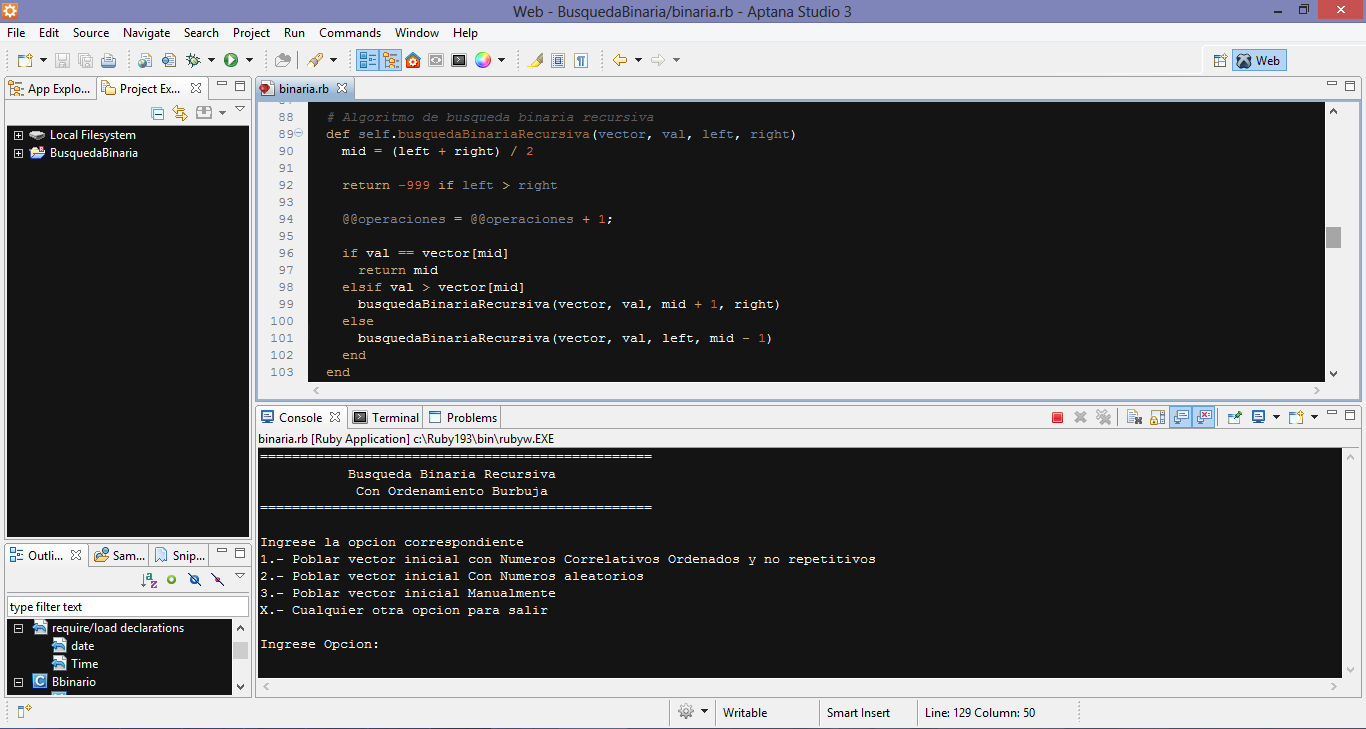
\includegraphics[scale=0.25]{Programa.png}
  				\caption{Pantallazo Aptana}
  				\label{fig:lls}
			\end{figure}	
	\end{frame}





\section{Conclusiones}
	\begin{frame}
		\frametitle{Conclusiones}
			\begin{itemize}[<+->]
				\item Se puede mejorar usando arboles autobalanceables, aunque estar asegurando minuciosamente puede añadir un costo considerable.
				\item No se nota la tendencia logaritmica de las inserciones debido a la complejidad lineal del recorrido.
			\end{itemize}
	\end{frame}



\end{document} 
